\documentclass[a4paper]{article}

\usepackage[english]{babel}
\usepackage[utf8]{inputenc}
\usepackage{amsmath}
\usepackage{graphicx}
\usepackage[colorinlistoftodos]{todonotes}
\usepackage{hyperref}

\title{Reinforcement learning for cache-friendly recommendations}

\author{Clément Bernard and Jade Bonnet }


\begin{document}
\maketitle

\begin{abstract}


\end{abstract}






\section{Introduction}

Radio applications (like Deezer, Spotify) use recommended algorithms to create playlists for the users that take into account the user's preferences and the relations between contents. Similarly, Youtube generates a sequence of videos guiding the user to a session. Nevertheless, these recommendation algorithms don't take into account the network (for instance the network latency).
We proposed to solve this issue by implementing reinforcement learning algorithms that take into account both the network and the preferences of the user. The reinforcement learning algorithms aim to learn from experience by interactions with the user. 


\section{Problem}

\paragraph{Catalogue} We consider that the user can choose a content among a catalogue $\cal{K}$ of size K. This catalogue can be adapted to different configurations like videos or musics. 
\paragraph{Recommendation System} To know which content is related to another, we assume a matrix $\cal{U} \in \cal{R}^{K \times K} $ where $u_{i,j} \in [0,1]$. Therefore, $u_{i,j} = 0$ means that the content $j$ isn't related to the content $i$ and $u_{i,j} = 1$ means that the content $j$ is highly related to the content $i$. \\
Furthermore, we also assume that we recommend only 1 content after the user has watched one.
\paragraph{Caching cost} Each content is associated with a cost, that can represent the network latency. For a content $i$, the cost associated is denoted $x_i \in \{0,1\}$. If a content is cached, the cost is $x_i = 0$ and whenever $x_i = 1$ the content is non-cached. 
\paragraph{User models} 
We model two different types of users.
\begin{enumerate}
    \item \textbf{Markovian User} : After this user has consumed a content i, he will : 
    	\begin{enumerate}
	\item Leave the simulation with probability $\alpha$
	\item Stay in the simulation with probability $1 - \alpha$ and :
	\begin{enumerate}
        \item Pick the content we offer to him with probability $a$
        \item Choose with probability $1 - a$ a content $j$ among the catalogue with probability $p_j$, where $p_j \in [0,1]$ and $\sum_{j=1}^{K}p_j = 1$. Therefore, it will ignore the recommender
        
        
    \end{enumerate}
		
	\end{enumerate}    
    
    
    \item \textbf{Specific User} : After this user has consumed a content i, he will :
    \begin{enumerate}
    	\item Leave the simulation with probability $\alpha$
	\item Stay in the simulation with probability $1 - \alpha$ and :  
	\begin{enumerate}
        \item Accept the content $j$ with probability $a_{i,j} = \frac{u_{i,j}}{max_i (u_i)}$
        \item Otherwise, he will choose a content $j$ like before : with probability $p_j$, where $p_j \in [0,1]$ and $\sum_{j=1}^{K}p_j = 1$. 
    \end{enumerate}
	
    \end{enumerate}
        
\end{enumerate}

\paragraph{Recommendation process}

We aim to solve a recommendation issue by interactions with the user. Indeed, by using reinforcement learning approach, the algorithm will interact with the user to learn how he works (like its preferences). Furthermore, the algorithm doesn't aim to only learn the user's behaviour : it will take into account the cached contents to create a trade-off between proposing cached content or related contents.

\section{Reinforcement learning algorithms}

\subsection{Definition}

\paragraph{Reinforcement learning} This is a subclass of machine learning, such as \textit{supervised learning} or \textit{unsupervised learning}. Reinforcement learning is learning how to map situations to actions in order to maximise rewards. The learner is not told which action to do, but should discover which action results in higher results by trying them. The challenges of reinforcement learning are the facts that a given action has impact in the immediate reward but in the next situation, and so the future rewards. Reinforcement learning is therefore a trade-off between learning by interaction and delayed rewards. 

\subsection{Elements of Reinforcement Learning}
	\subsubsection{Markov Decision Processes}
	The finite Markov Decision Processes (MDPs) are a classical way to model sequential decision making, where the actions influence not immediate rewards but also future states and rewards. It helps us to create a mathematical model for our problem. \\
A reinforcement learning system has several main elements that include an Agent, Environment, State, Action, Reward, Policy, and Value Function.
\paragraph{Agent}The learner that will make the decisions, of what actions to take. In this case the agent is the algorithm of recommendation. The decisions he will take at time t is noted $A_t$
\paragraph{Environment} Things that interact with the Agent. It will interact with the agent by returning a Reward $R_{t+1}$ and the next States $S_{t+1}$. In our case, the environment is the user himself.  
\paragraph{Reward}  Feedback on the actions taken by the agent, it can measure the success or failure of the actions taken. In our case, we give positive rewards if the content we suggest is either related or cached.
\paragraph{Action} Content that is suggesting by the agent. This is an element among the catalogue $\cal{K}$. 
\paragraph{State} Content that is currently consumed by the environment (user). This is also an element among the catalogue $\cal{K}$. 




\paragraph{} In a MDP, the goal of the agent is to learn what actions will lead to best rewards through a finite sequence of interaction with the environment. 

\begin{figure}[h!]
\begin{center}
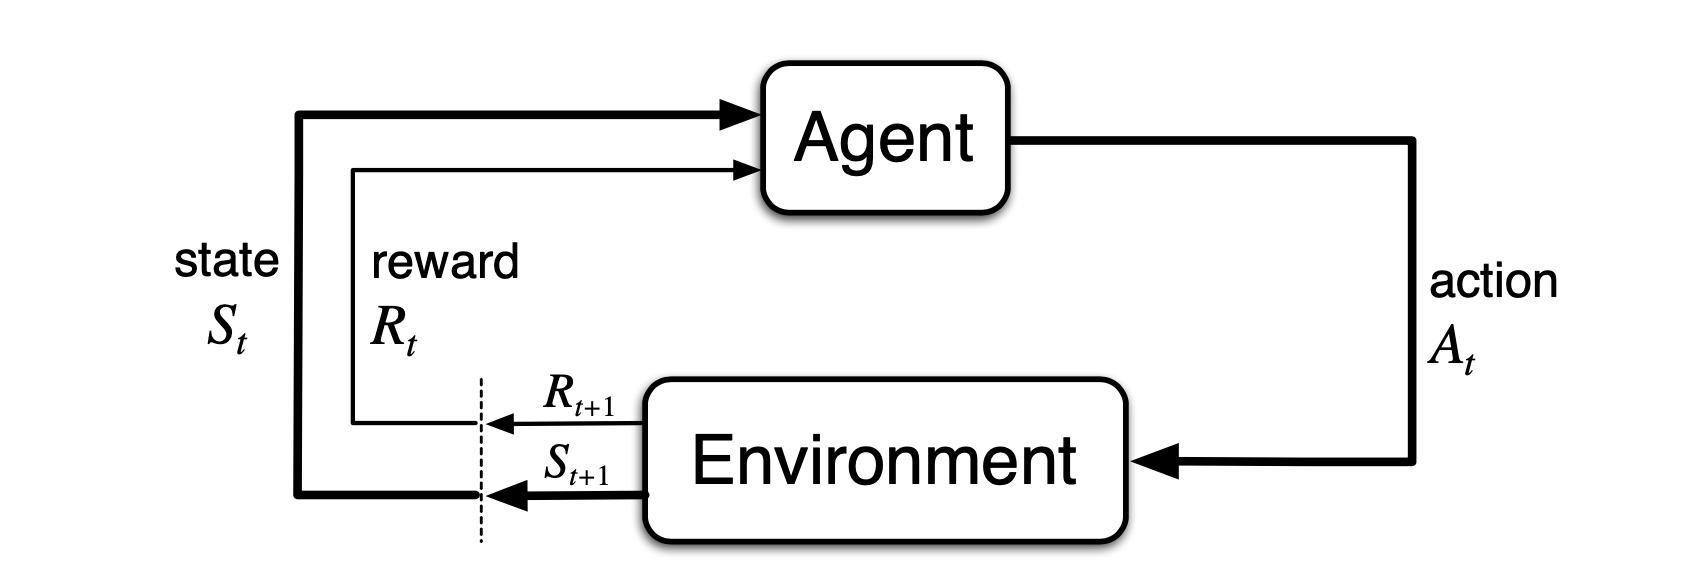
\includegraphics[width=0.8\linewidth]{img/mdp.png}
\caption{Agent-environment interaction in a MDP}
\end{center}
\end{figure}

\paragraph{} The agent and the environment will interact at each sequence of time t = 0,1,2,3,4,... At each timestep t, the agent receives a state $S_t$ and will offer an action $A_t$ from what he knows. Then, the environment, as a result of this action, will return a reward $R_t$ to this action and lead the agent to a new state $S_{t+1}$. \\
It leads to a trajectory like this : 
\[ S_0, A_0,  R_1, S_1, A_1, R_2, S_2, A_2, ... \]
In our problem, a timestep corresponds to a content that is consumed (for instance a video or a music for example).
\paragraph{State-transition probability} With the previous notations, we can define a state-transition probability which describe the probability to be in a next state $S_{t+1}$ given the current state $S_t$ and an action $A_t$ : 

\[ P(S_{t+1} = j | S_t = i, A_t = k ) =  \left \{
   \begin{array}{r c l}
      (1-\alpha)a  \quad  if \quad j = k \\
      (1-\alpha)(1-a)p_j  \quad  if \quad j \ne k \\
      
   \end{array}
   \right .
				  \]

	\subsubsection{Returns, policy and value function}

So far we have defined our problem in term of MDPs, but we haven't defined yet the objective of the learner. 

\paragraph{Return} This is the cumulative sum of the rewards from step t. It is defined as follow : 
\[
G_t =  R_{t+1} + R_{t+2} + ... + R_{T} 
\] where T denotes the timestep where the simulation ends (the user has left the simulation for instance). \\
\paragraph{Expected return} The previous formulation of the return doesn't take into account the fact that a current reward could have high impact at time t that the one at time T. To cope with it, we add a \textbf{discount} factor $\gamma$ with $0 \le \gamma \le 1$. The expected reward is then defined as : 
\[  G_t = R_{t+1} + \gamma R_{t+2} + \gamma^ 2 R_{t+3} + ... + \gamma^{T-1} R_{T} = \sum_{k=0}^{T}\gamma^k R_{t+k+1}            \]
The discount factor $\gamma$ represents the value of future rewards : $\gamma = 0$ means the agent is 'myopic' and only considers maximizing current rewards whereas if $\gamma$ is close to 1, the agent takes into account future rewards. 


\paragraph{Policy } Mapping from states to probabilities of selecting an action. If an agent is following a policy $\pi$ at time t, then $\pi(a|s)$ gives the probability of choosing the action $A_t = a$ from state $S_t = s$.

\paragraph{Value function} The value function of a state s under a policy $\pi$, denoted as $v_{\pi}(s)$ is defined as the expected return when starting from the state s and following the policy $\pi$ :  
\[ 
v_{\pi}(s) = E_{\pi}(G_t | S_t = s) 
\]
\paragraph{Action-value function} As described above, we define the value of taking action a in state s under a policy $\pi$, denoted $q_{\pi}(s,a) $, as the expected return from state s, taking the action a and following the policy $\pi$ : 
\[ q_{\pi}(s,a) = E_{\pi}(G_t | S_t = s, A_t = a) \] 


\subsection{Q-Learning}

\subsubsection{Optimality}

\paragraph{} There are different policies that can handle a reinforcement learning problem. Nevertheless, some policies are better than others. But what does better mean in MDP ? 
\paragraph{Order in term of policy} A policy $\pi$ is better than a policy $\pi'$ if its expected return is greater than or equal to that of $\pi'$ for each state.
\paragraph{Optimal policy} There is always at least one policy which is greater than or equal to every other policies. Same idea for the action-value function. We denote them as follow : 
\[    v_{*}(s) = \max_{\pi} v_{\pi}(s)          \] and 
\[    q_{*}(s,a) = \max_{\pi} q_{\pi}(s,a)          \] 


\subsubsection{Bellman optimality equations}

The Bellman equations express the relationships between the value of a state and the value of the next states. 
Furthermore, the Bellman optimality equations express the fact that the value of a state under an optimal policy should be equal to the expected return for the best action from that state : 
\[  v_{*}(s)  = \max_{a} q_{\pi_{*}}(s,a)   = \max_{a} \sum_{s',r} p(s',r | s,a) [r + \gamma v_{*}(s')]                \]
There is the equivalent equation for the state action value function : 
\[  q_{*}(s,a) = \sum_{s', r} p(s',r |s,a) (r + \gamma \max_{a'} q_{\pi}(s',a')    )        \]
This is actually a system of equations for each state. \\
Once the optimal function of state-action pairs is determined, one can infer the optimal action to take from a given state s  : 
\[   argmax_{a'} q_{*}(s,a')                \]
Therefore, after determination of the optimal Q table, we know which content to recommend for the user for each content in the catalogue.

\subsubsection{Q learning algorithm}
\paragraph{} To learn how to approximate the optimal state action pairs, we can approximate directly $q_{*}$. To do so, we use this following formula : 

\[   Q_{t+1}(S_t, A_t) =   Q_{t}(S_t, A_t) + \alpha (R_{t+1} + \gamma \max_{a} Q(S_{t+1} , a) - Q_{t}(S_t, A_t)        )            \]

It leads to the Q learning algorithm : 

\begin{figure}[h!]
\begin{center}
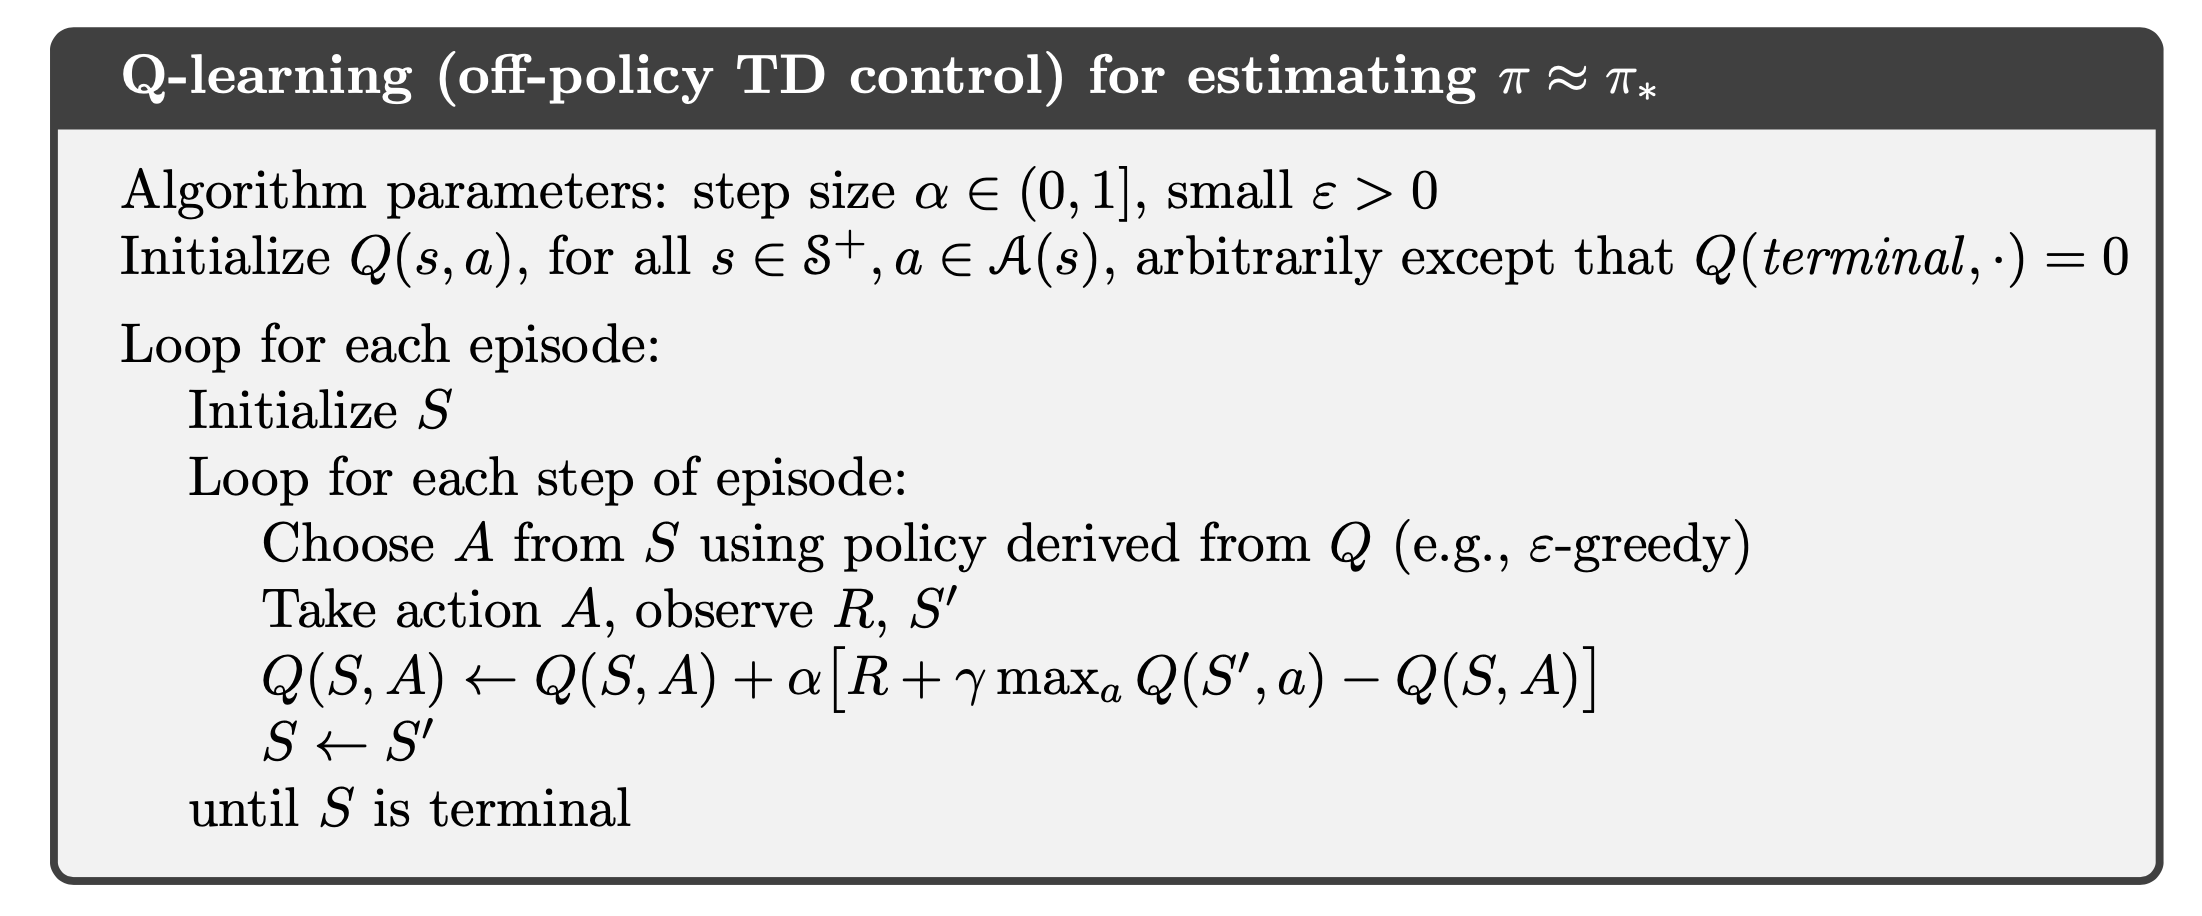
\includegraphics[width=1.2\linewidth]{img/qlearning.png}
\caption{Q learning algorithm}
\end{center}
\end{figure}

\newpage

\subsubsection{Exploration and Exploitation ($\epsilon$-greedy)}


In the above algorithm, the selection of an action by the agent (and so the content to recommend) is chosen in a specific way. Indeed, there is a trade-off between : 
	\begin{enumerate}
		\item \textbf{Exploration} : with probability $\epsilon$, the agent will pick randomly a content among the catalogue. The purpose is to enable the agent to continue to explore the possible actions in order not to avoid some decisions.  
		\item \textbf{Exploitation} : with probability $1 - \epsilon$, the agent will pick the action that maximises the q values : $argmax_{a}  Q(S_t, a)   $
	\end{enumerate}
This is very important to keep this trade-off : avoiding the exploitation will lead to random recommendations whereas avoiding the exploration will lead to eventually bypass good actions. \\
Furthermore, one can consider to start with a high $\epsilon$ to advantage the exploration (because we have no knowledge of the expected rewards yet) and then gradually decreasing the $\epsilon$ as the agent learns more and more about the environment.\\
 Nevertheless, we don't consider this approach because it is equivalent to assume that the user doesn't change and he will keep his preferences. We don't want to assume these and so we keep $\epsilon$ constant.  
    
    
\subsubsection{Convergence criteria}
There are two ways to consider the end of the algorithm, and therefore to get the final Q values (which should correspond to the optimal Q values) : 
	\begin{enumerate}
		\item \textbf{Number of epochs} : We simulate user experiences and in the same time we update the q-table for a number of times predefined. Then, we risk to have situation where the q-table values don't update anymore and we compute for nothing.
		\item \textbf{Threshold} : We use a criteria to say whether the Q-table values have converged. To do so, we consider the maximum difference of q-tables values over an episode. That is to say, we let the user consume contents, and whenever he has terminated, we take the maximum difference between the previous q-table and the new one obtained after the simulation. If this value is less than a threshold (new hyperparameter), then we stop the process and we consider the q-tables as optimal.
	\end{enumerate}
    
    
 \subsubsection{Hyperparameters}
 There are some hyperparameters to take into account in the Q learning algorithm. 
 \begin{enumerate}
 	
	\item \textbf{Learning rate } $\alpha$ : it describes how fast we want to adjust the q values. This is as a classic supervised algorithm with gradient descent : a too high value of $\alpha$ leads to diverge whereas a too low value leads to increase the convergence time. 
 	\item \textbf{Discounted } $\gamma$ : It deals with the rewards that the agent considers to update the Q values. Indeed, if $\gamma = 0$ the agent will prefer actions with high current rewards whereas $\gamma$ close to 1 will lead the agent to consider actions that lead to future high rewards. For instance, if $\gamma = 0.9$, it will take into account 10 future episodes.
	
 \end{enumerate}
 
 	Furthermore, there are also hyperparameters for the environment (and so the user we use). If the user is a Markovian one, the hyperparameters are the following : 
	
	\begin{enumerate}
	
	\item \textbf{Cached contents} : Number of cached contents. This is what takes into account the network : the cached contents shouldn't cost anything to the user in order to consume it. On the other hand, a non-cached content can, if this is a popular one, lead to latency and decrease the user's experience.
	\item \textbf{Related contents} : Number of related contents for each state. For instance, if the catalogue is a list of music, the related contents can be musics from same genre or artist. We keep this number constant for each state, and it shouldn't be more than 10  percent of the total size of the catalogue.
	\item $\alpha$ : Probability to leave the experience. It corresponds to the end of a user experience. For instance, it could correspond to the time spent on Youtube watching consecutive videos.
	\item \textbf{a} : Probability that the user follows our recommendations. This coefficient is set constant for sake of simplicity, but should evolve through the process. Indeed, if we recommend contents that the user dislikes, he won't trust the recommender and so will choose himself the future contents.    
	\end{enumerate}
	Note that for the specific user described above, the only difference is in the a coefficient. 


\subsection{Results}

	\subsubsection{Q-table}
	
	We tried to solve two different problems : 
		\begin{enumerate}
			
			\item \textbf{Classic recommender} : In the exploration part, we consider all the contents with uniform probability.
			\item \textbf{Restricted recommender} : In the exploration part, we only consider the related contents (we use the non null values in the U matrix).
			
		\end{enumerate}
	Hence, we expect different behaviour for the final q-table.  \\
	We also consider that a content that is related and cached will lead to a reward of +2, whereas a content that is either related or cached will lead to a reward of +1. Finally, a content neither related nor cached will lead to a reward of 0. \\
	Here are the results of a q-table after applying the Q-learning algorithm for 100 000 epochs , with a random U matrix and cached list : 
	
	
	
	
	To understand what these plots mean, it requires to read it line by line. In fact, for a given state (a line in these plots), the values we got in this line are the expected rewards for recommending this action (content). We can see that, as the cached contents are fixed, the vertical lines correspond to these contents. The expected rewards are usually high as the immediate reward, whatever state the environment is,  is +1. Moreover, whenever a q_value is yellow (which means the q value associated is very high), the content is usually related and cached. \\
	Note that the recommendation strategies are really different for different values of gamma.
	 
	
	\subsubsection{Discounted \gamma parameter}
	To understand the role of $\gamma$, we can focus on the optimal Q functions obtained for extreme values of $\gamma$.
	Here is the result, with the same environment defined above : 
	
	
	
	
	
	
	On one hand, the q-table for $\gamma = 0 $ if predictable. This can be found with both the U matrix and the cached list. Indeed, it only consider immediate rewards, which is directly linked to the fact that a content is either related or cached.  \\
	On the other hand, for $\gamma = 0.9$, we see that this is more noisy. The Q-table values are very close. As it considers future rewards, even a not cached and not related content can lead to high rewards. That's why the values are so close. \\
	 
	\subsubsection{Constrained exploration}
	As mentionned above, we implemented a version of the exploration part where we only consider the related contents. It means that we don't consider the contents that are neither related nor cached (which makes sense because a user won't probably enjoy watching a video that has latency and isn't related at all to his current video). Here is the result obtained, with the same environment described previously.




\subsection{Deep Q-learning}





\begin{thebibliography}{99}

\bibitem{Bostrom}
Bostrom, Nick. 2014. \textit{Superintelligence: Paths, Dangers, Strategies.} New York: Oxford University Press.


\end{thebibliography}











\end{document}